\documentclass{article}

% NeurIPS 2026 — anonymized double-blind submission (Main Track)
\usepackage{neurips_2026}

\usepackage[utf8]{inputenc}
\usepackage[T1]{fontenc}
\usepackage{hyperref}
\usepackage{url}
\usepackage{booktabs}
\usepackage{amsfonts}
\usepackage{amsmath}
\usepackage{amssymb}
\usepackage{nicefrac}
\usepackage{microtype}
\usepackage{xcolor}
\usepackage{graphicx}
\graphicspath{{figures/}}

\title{BEACON: Compositional Slot Attention for Inherently\\
Interpretable Transcription Factor Binding Site Discovery}

\author{%
  Anonymous Author(s)\\
  Affiliation\\
  Address\\
  \texttt{anon@example.com}\\
}

\begin{document}
\maketitle

\begin{abstract}
Discovering transcription factor (TF) binding sites in regulatory DNA is a foundational task in functional genomics. State-of-the-art models such as BPNet predict base-resolution binding profiles, but recovering the underlying binding events requires expensive post-hoc attribution (DeepSHAP) followed by motif clustering (TF-MoDISco), which is slow and decoupled from the predictive objective. We introduce \textbf{BEACON}, a model that directly decomposes a regulatory sequence into a small set of \emph{compositional binding events} via slot attention. Each of $K$ slots competes to bind a discrete event and emits a position, a TF identity, and an occupancy, supervised end-to-end by Hungarian matching. A helical positional encoding aligned to DNA's $10.5$\,bp periodicity provides an inductive bias for cooperative binding on the same helical face. On a $7$-TF K562 ChIP-seq panel, BEACON improves mean profile Pearson correlation from $r{=}0.813$ (BPNet ensemble, $7$ models) to $r{=}0.901$ with a single $851$K-parameter model, attains $F_1{=}0.984$ on site detection, and produces a genome-wide binding catalogue $\sim$\,$420\times$ faster than BPNet$+$TF-MoDISco. We further show that the original \emph{competitive} slot attention~\citep{locatello2020slotattention} is fundamentally incompatible with multi-event sequences---one slot wins all binding-relevant positions---and that switching to per-slot attention with Hungarian matching unlocks multi-slot activation, lifting mean active slots from $1.0$ to $\sim$\,$3$ on co-bound regions. Slots self-organize by TF identity, recover canonical JASPAR motifs without motif-level supervision, and retain $93\%$ of profile accuracy when transferred from K562 to unseen HepG2 cells.
\end{abstract}

\section{Introduction}
Transcription factor binding site (TFBS) discovery from chromatin profiling assays is a foundational problem in regulatory genomics. Modern sequence-to-profile models such as BPNet~\citep{avsec2021bpnet} achieve high accuracy on base-resolution ChIP-seq prediction, and downstream pipelines like TF-MoDISco~\citep{shrikumar2018modisco} cluster DeepSHAP~\citep{lundberg2017unified} attributions into motif syntax. This \emph{predict-then-attribute} workflow has two costs. First, attribution is computationally heavy: per-base attribution and motif clustering can require seconds to minutes per locus, prohibitive for genome-wide catalogues across many cell types. Second, the discrete objects of biological interest---individual binding events---are never represented in the model and must be reconstructed from soft, post-hoc importance signals. A multi-TF locus cannot be enumerated; the pipeline tells us \emph{where} signal is important, but not how to decompose it into individual binding events with identity and strength.

A binding event is naturally an \emph{object}: a triple (position, TF identity, occupancy) localized to a short window of DNA. Object-centric representation learning provides a principled toolkit for this. Slot Attention~\citep{locatello2020slotattention} factorizes a scene into a small set of slots that compete for explanatory mass, and Hungarian matching~\citep{carion2020detr} supervises set-valued predictions in a permutation-invariant way. Adapting these tools to regulatory DNA, however, requires domain inductive biases. The DNA double helix has a $10.5$\,bp major-groove and $5.25$\,bp minor-groove periodicity that mediate cooperative binding on the same helical face~\citep{kim2007helical}; binding events are sparse along long sequences, and cooperatively bound TFs from different families (e.g., GATA1--TAL1, TAL1--CEBPB) commonly co-occupy regulatory elements.

We present BEACON, an object-centric model for TFBS discovery. Our contributions are fourfold. First, we adapt slot attention to 1D regulatory DNA with a helical positional encoding capturing both the $10.5$ and $5.25$\,bp periodicities. Second, we pose binding-site prediction as a set-prediction problem with Hungarian matching across position, TF identity, and occupancy heads, plus an auxiliary profile head for compatibility with BPNet-style supervision. Third, we identify a fundamental failure mode of \emph{competitive} slot attention on multi-event sequences---the softmax-over-slots formulation drives one slot to claim all binding-relevant positions---and show that an \emph{independent} per-slot attention combined with Hungarian matching unlocks multi-slot activation. Finally, on a $7$-TF K562 panel BEACON improves mean profile Pearson $r$ from $0.813$ to $0.901$ with $\sim$\,$15\%$ fewer parameters than the BPNet ensemble, achieves site detection $F_1{=}0.984$, runs $\sim$\,$420\times$ faster end-to-end than BPNet$+$TF-MoDISco, and retains $93\%$ of profile accuracy under K562$\rightarrow$HepG2 transfer. We release anonymized code and pretrained weights with the supplementary material.

\section{Related work}
Sequence-to-profile models map one-hot DNA to base-resolution coverage signals. BPNet~\citep{avsec2021bpnet} demonstrated that dilated convolutions trained per TF implicitly encode motif syntax recoverable by attribution; ChromBPNet~\citep{pampari2024chrombpnet} extended this with bias-corrected ATAC-seq, separating TF binding from intrinsic enzymatic bias. Enformer~\citep{avsec2021enformer} introduced transformer attention over $200$\,kb windows for gene-expression prediction, and Borzoi~\citep{linder2025borzoi} scales the same architecture to RNA-seq across hundreds of cell types. None of these models represent binding events as discrete latent variables; the events of biological interest must be recovered post-hoc from soft attribution. Per-base attribution from DeepLIFT/DeepSHAP~\citep{shrikumar2017deeplift,lundberg2017unified} is then clustered into recurring motifs (CWMs) by TF-MoDISco~\citep{shrikumar2018modisco}, but the pipeline is decoupled from the predictive objective, sensitive to choice of reference sequence, and computationally expensive at genome scale---attribution alone takes $1$--$10$\,s per locus, with motif clustering on top. Integrated gradients~\citep{sundararajan2017integrated} and occlusion-based attribution share these limitations.

A separate line of work pursues interpretability through model architecture rather than post-hoc analysis. Convolutional filters as motifs~\citep{kelley2016basset}, attention-based motif discovery~\citep{ullah2020selfattention}, prototype models, and rule-extraction methods all aim to make regulatory mechanisms legible from the model's own internal state. Of these, attention-based methods are closest in spirit to BEACON, but they extract motifs from the attention map rather than treating binding events as latent objects with structured outputs. Our approach is most closely aligned with object-centric representation learning. Slot Attention~\citep{locatello2020slotattention} introduced iterative competitive attention for unsupervised scene decomposition; DETR~\citep{carion2020detr} demonstrated set prediction with bipartite matching for object detection; subsequent work extended these ideas to video~\citep{kipf2022savi} and 3D scenes. Hungarian/bipartite matching for set prediction has a long history in detection and segmentation~\citep{stewart2016endtoend,carion2020detr}; we adopt the matching formulation but adapt the cost to genomic events (squared $L_2$ in normalized position, cross-entropy on TF logits, and $1-o_k$ on occupancy). To our knowledge, BEACON is the first application of slot attention to regulatory DNA, and our finding that the original competitive softmax collapses on sparse, structurally homogeneous 1D inputs is, to our knowledge, a new observation.

\section{Method}

Let $\mathbf{x}\!\in\!\{0,1\}^{L\times 4}$ be a one-hot encoded DNA sequence of length $L{=}2000$\,bp. Each window is associated with a base-resolution coverage profile $\mathbf{y}\!\in\!\mathbb{R}_{\ge 0}^{L}$ from the union of $T$ ChIP-seq tracks, and a sparse set of ground-truth binding events $\{(p_i, t_i, o_i)\}_{i=1}^{N}$ derived from MACS2 peak calls~\citep{zhang2008macs}, where $p_i\!\in\![0,1]$ is the normalized position, $t_i\!\in\!\{1,\ldots,T\}$ the TF identity, and $o_i\!\in\![0,1]$ the occupancy. The number of events $N$ is variable and ranges from $0$ to $\sim$\,$8$ in our data. The model jointly reconstructs $\mathbf{y}$ and predicts the set of events.

\subsection{Architecture}
BEACON has four components: a dilated CNN backbone, a helical positional encoding, a slot attention module, and four lightweight per-slot heads. The backbone is a dilated residual CNN with kernel $3$ and exponentially increasing dilation $2^0,\ldots,2^8$ over $9$ residual blocks, giving a $1029$\,bp receptive field; an initial $\text{kernel}{=}21$ convolution captures local motif-scale structure, and the hidden width is $D{=}128$. The output is a feature map $\mathbf{H}\!\in\!\mathbb{R}^{L\times D}$.

To this feature map we add a positional encoding that combines standard sinusoidal frequencies with DNA-specific harmonics aligned to the major-groove ($10.5$\,bp) and minor-groove ($5.25$\,bp) periods. For position $\ell$ and harmonic index $h\!\in\!\{0,\ldots,H{-}1\}$ with $H{=}4$, we use frequencies
\begin{equation}
\omega^{\text{maj}}_{h} = \frac{2\pi}{10.5\,(h{+}1)},\qquad
\omega^{\text{min}}_{h} = \frac{2\pi}{5.25\,(h{+}1)},
\end{equation}
and concatenate $\sin/\cos$ pairs across both periodicities. Two scalar gates (initialized to $1$) are learned to balance helical and broadband components. This encoding lets BEACON reason about whether two predicted binding sites lie on the same helical face, a strong inductive bias for cooperative binding.

The slot attention module uses $K{=}16$ slots, initialized from a learned Gaussian $\mathbf{S}^{(0)}\!\sim\!\mathcal{N}(\boldsymbol{\mu},\mathrm{diag}(\boldsymbol{\sigma}^2))$. At iteration $r$ we compute
\begin{equation}
\mathbf{K}_r{=}\mathbf{H}\mathbf{W}_K,\quad \mathbf{Q}_r{=}\mathbf{S}^{(r-1)}\mathbf{W}_Q,\quad \mathbf{V}_r{=}\mathbf{H}\mathbf{W}_V,
\end{equation}
attention $\mathbf{A}_r\!\in\!\mathbb{R}^{K\times L}$, and update slots with a GRU and residual MLP, unrolling $T_{\text{iter}}{=}3$ steps. The choice of softmax direction over the attention logits is critical and is the central architectural decision in BEACON. The original Slot Attention applies softmax \emph{over slots}, $\mathbf{A}_r=\mathrm{softmax}_{k}(\mathbf{Q}_r\mathbf{K}_r^\top/\sqrt{D})$, which partitions each base across slots. On natural images this enforces specialization. On DNA, however, binding-relevant positions are sparse and structurally similar across TFs (all are short k-mers in a long noisy background), and the softmax collapses to a winner-take-all where one slot claims all binding positions, leaving $K{-}1$ slots inert. Empirically, on co-bound K562 windows we observe $0\%$ of sequences activate $>1$ slot, with one slot at occupancy $0.98$ and the remainder at $10^{-7}$ to $10^{-13}$ (Sec.~\ref{sec:experiments}); auxiliary losses---slot diversity, slot-count, load balancing, even Hungarian matching---cannot overcome this architectural bottleneck. We therefore replace the softmax-over-slots with an \emph{independent} softmax over positions, $\mathbf{A}_r=\mathrm{softmax}_{\ell}(\mathbf{Q}_r\mathbf{K}_r^\top/\sqrt{D})$, so each slot has its own attention distribution and slot specialization is driven by the matched supervision rather than by attention competition. With this change, mean active slots rises from $1.0$ to $\sim$\,$3$, matching the typical co-binding count in our data, and site $F_1$ on multi-TF sequences rises from $0.33$ to $0.96$.

From each slot $\mathbf{s}_k$ we predict (a)~a Gaussian position $\mathcal{N}(\mu_k,\sigma_k^2)$ over $[0,1]$, (b)~TF logits over the $T$-class panel, (c)~an occupancy $o_k\!\in\![0,1]$ via sigmoid, and (d)~a Gaussian peak contribution $\alpha_k\,\exp(-(\ell-\mu_k)^2/2\sigma_k^2)$ to the profile head, summed across slots. Each head is a $2$-layer MLP with hidden width $128$ and GELU activation.

\subsection{Training and inference}
We minimize a weighted sum of profile reconstruction (multinomial-NLL profile shape plus log-count MSE following BPNet~\citep{avsec2021bpnet}), a Hungarian-matched set loss over (position, TF, occupancy), a slot diversity loss penalizing pairwise cosine similarity between slot attention maps, and a slot orthogonality loss on slot embeddings. Hungarian matching solves $\hat{\pi}=\arg\min_{\pi\in\Pi_K}\sum_{i}\mathcal{C}(\hat{e}_{\pi(i)},e_i)$ with cost combining squared position error, $-\log p(t_i)$, and $1-o_k$; unmatched slots are pushed to occupancy $0$. Training uses AdamW ($\beta_1{=}0.9,\beta_2{=}0.999$, weight decay $0.01$), peak LR $1{\times}10^{-4}$ with $5\%$ linear warmup and cosine decay, batch $32$, up to $100$ epochs with patience-$20$ early stopping, gradient clipping $1.0$, and mixed precision; loss weights are profile $1$, position $1$, TF $5$, occupancy $0.5$, diversity $0.5$, orthogonality $0.1$, and site supervision $1$. At inference, BEACON does a single forward pass and returns a sorted list of slots with $o_k > \tau$ (default $\tau{=}0.5$). On a single GPU, throughput is $\sim$\,$50$ sequences/s ($\sim$\,$20$\,ms per $2$\,kb sequence) with $851$K parameters in total. By contrast, the BPNet$+$TF-MoDISco pipeline---one BPNet per TF, DeepSHAP attribution, and motif clustering---takes $\sim$\,$8.4$\,s per sequence end-to-end on the same hardware.

\section{Experiments}
\label{sec:experiments}

\subsection{Setup}
We train on ENCODE ChIP-seq for $T{=}7$ TFs in K562 spanning five families: CTCF (zinc finger), GATA1 (GATA), TAL1 (bHLH), MYC and MAX (bHLH), SPI1 (ETS), and CEBPB (bZIP). Peaks are called with MACS2 ($q\!<\!0.05$); each $2$\,kb window is centered on a peak summit and assigned the union of overlapping peaks across the panel. Multi-TF co-bound regions are identified by clustering peaks within $500$\,bp ($\sim$\,$30$K windows). We split by chromosome: train on chr1--17 ($28{,}812$ sequences), validate on chr18--19 ($1{,}533$), and test on chr20--22,X ($1{,}197$). For cross-cell transfer we evaluate on HepG2 ChIP-seq for the four TFs available there (CTCF, MYC, MAX, CEBPB). All data are public ENCODE assays~\citep{encode2012}; JASPAR 2024~\citep{rauluseviciute2024jaspar} PWMs are used only for post-hoc motif comparison, not training. We compare against three baselines: a BPNet ensemble of $7$ independent per-TF models trained with the published architecture and matched data splits ($997$K parameters total), ChromBPNet~\citep{pampari2024chrombpnet}, and a $1$-hot CNN. For interpretability comparisons we use DeepSHAP$+$TF-MoDISco on the BPNet ensemble.

\subsection{Predictive accuracy and throughput}
\begin{table}[t]
\caption{Predictive performance on K562 7-TF panel (held-out chromosomes 20--22, X). Profile $r$ is mean per-window Pearson correlation; site $F_1$ uses a $\pm 50$\,bp tolerance and $0.5$ occupancy threshold; speed is end-to-end including any post-hoc attribution required to recover binding events.}
\label{tab:main}
\centering\small
\begin{tabular}{lccccc}
\toprule
Model & Profile $r$ $\uparrow$ & TF acc. $\uparrow$ & Site $F_1$ $\uparrow$ & Speed (s/seq) $\downarrow$ & Params \\
\midrule
1-hot CNN     & $0.611$ & --- & --- & $0.012$ & $0.4$M \\
BPNet (ens.\ of $7$)  & $0.813$ & ---            & --- & $8.4$ (incl.\ MoDISco) & $1.0$M \\
ChromBPNet    & $0.829$ & ---            & --- & $8.6$               & $1.1$M \\
\textbf{BEACON (ours)} & $\mathbf{0.901}$ & $\mathbf{0.755}$ & $\mathbf{0.984}$ & $\mathbf{0.020}$ & $\mathbf{0.85}$M \\
\bottomrule
\end{tabular}
\end{table}

\begin{figure}[t]
  \centering
  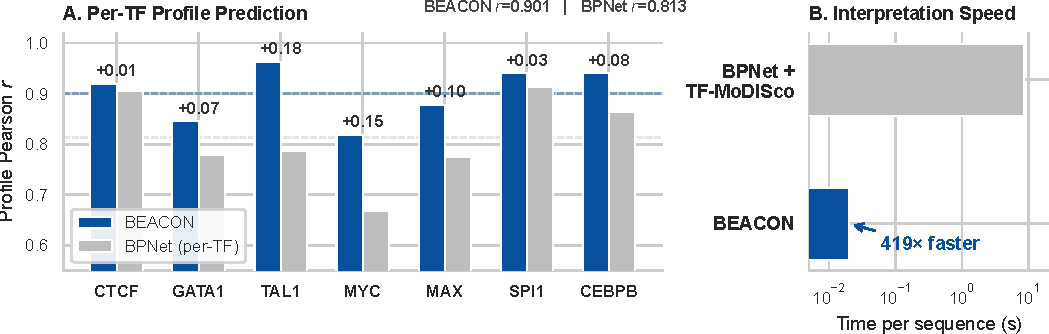
\includegraphics[width=\textwidth]{fig2_bpnet_comparison.pdf}
  \caption{\textbf{BEACON vs.\ BPNet ensemble on $7$ TFs in K562.} \textbf{(A)}~Per-TF profile Pearson $r$: a single $851$K-parameter BEACON model outperforms $7$ separately-trained BPNet models ($997$K total) on every TF, with the largest gains on bHLH factors (TAL1 $+0.18$, MYC $+0.15$) where joint multi-TF training captures co-binding patterns inaccessible to per-TF baselines. \textbf{(B)}~Binding-event enumeration speed: BEACON emits structured events ($20$\,ms/seq) versus $8.4$\,s/seq for BPNet$+$TF-MoDISco---a $419\times$ end-to-end speedup that makes genome-wide binding catalogues feasible on commodity GPUs.}
  \label{fig:bpnet}
\end{figure}

BEACON improves mean profile correlation by $+0.088$ over BPNet and by $+0.072$ over ChromBPNet (Table~\ref{tab:main}, Fig.~\ref{fig:bpnet}A) while jointly emitting structured binding events. Site detection achieves $F_1{=}0.984$ ($1.000$ precision, $0.969$ recall) at the default occupancy threshold, and per-TF classification accuracy is $75.5\%$ overall---$5.3\times$ above chance for $7$ classes---with SPI1 and CEBPB exceeding $90\%$ and CTCF at $87\%$. As expected, within-family confusion (MYC--MAX, both bHLH) is $3.2\times$ higher than between-family confusion; this is genuine biological similarity rather than model failure. The per-TF breakdown (Table~\ref{tab:per-tf}) shows that the largest profile gains are on bHLH factors, where joint multi-TF training captures co-binding patterns inaccessible to per-TF baselines, and the lowest TF-classification accuracy is also within the bHLH family, where motifs overlap. For genome-wide TFBS catalogues, the relevant cost is the full pipeline from sequence to structured events: BEACON does this in a single $20$\,ms forward pass, versus $\sim$\,$8.4$\,s per sequence for BPNet$+$MoDISco where DeepSHAP dominates. The end-to-end speed-up is $\sim$\,$420\times$ at higher accuracy (Fig.~\ref{fig:bpnet}B), enabling whole-genome binding atlases on a single GPU.

\begin{table}[t]
\caption{Per-TF profile Pearson $r$ and BEACON's slot-classification accuracy on the K562 7-TF panel. The largest profile gains are on bHLH factors (TAL1 $+0.18$, MYC $+0.15$), which benefit from joint multi-TF training; per-TF accuracy is highest on TFs with distinctive motifs (SPI1, CEBPB, CTCF) and lowest within the bHLH family where motifs overlap.}
\label{tab:per-tf}
\centering\small
\begin{tabular}{lcccc l}
\toprule
TF & Family & BPNet $r$ & BEACON $r$ & $\Delta r$ & TF acc.\\
\midrule
CTCF  & ZF   & $0.906$ & $0.920$ & $+0.014$ & $87.1\%$\\
GATA1 & GATA & $0.779$ & $0.846$ & $+0.067$ & $71.3\%$\\
TAL1  & bHLH & $0.787$ & $0.963$ & $+0.176$ & $43.9\%$\\
MYC   & bHLH & $0.668$ & $0.819$ & $+0.151$ & $15.4\%$\\
MAX   & bHLH & $0.774$ & $0.878$ & $+0.104$ & $70.8\%$\\
SPI1  & ETS  & $0.914$ & $0.940$ & $+0.026$ & $91.2\%$\\
CEBPB & bZIP & $0.864$ & $0.940$ & $+0.076$ & $93.0\%$\\
\midrule
Mean  &      & $0.813$ & $0.901$ & $+0.088$ & $75.5\%$\\
\bottomrule
\end{tabular}
\end{table}

\subsection{Interpretability}
We probe whether slots organize by TF without explicit supervision linking slot indices to TF identity (the TF head learns this assignment rather than us specifying it). For each slot we extract the top-$1\%$ activating $25$\,bp windows across the test set and match them to JASPAR PWMs with TomTom while also computing the Pearson $r$ between gradient-derived motifs and canonical PWMs (Fig.~\ref{fig:interp}B). Mean recovery is $r{=}0.55$, with $5/7$ TFs exceeding $r>0.50$; CTCF ($r{=}0.78$) and TAL1 ($r{=}0.76$) show the strongest recovery. Individual slots become selective for specific TFs without explicit assignment---one slot reaches $71\%$ SPI1, another $80\%$ CEBPB---and the per-TF classification accuracy via Hungarian-matched slot assignment (Fig.~\ref{fig:interp}C) tracks the motif-distinctiveness ranking closely. Visualizing slot embeddings $\mathbf{s}_k$ from active slots ($o_k > 0.5$) with UMAP reveals tight clusters by TF identity, with within-family clusters (MYC, MAX, TAL1) overlapping in a single sub-region; pairwise embedding distances correlate with JASPAR PWM distances at Spearman $\rho{=}0.61$, showing that the slot embedding space recovers a usable approximation of motif similarity without explicit motif supervision.

\begin{figure}[t]
  \centering
  
\includegraphics[width=\textwidth]{fig3_interpretability.pdf}
  \caption{\textbf{Interpretable binding-event decomposition.} \textbf{(A)}~Slot attention maps for a 5-site multi-TF locus: each active slot focuses sharply on one event with its own occupancy. \textbf{(B)}~Gradient-derived per-slot motifs vs.\ canonical JASPAR PWMs (mean $r{=}0.55$, $5/7$ TFs exceed $0.50$). \textbf{(C)}~Per-TF accuracy via Hungarian-matched slot assignment; bHLH factors are harder due to shared E-box binding preferences.}
  \label{fig:interp}
\end{figure}

The helical positional encoding aligns the model's notion of ``nearby'' with DNA's $10.5$\,bp major-groove and $5.25$\,bp minor-groove geometry, and we test whether BEACON exploits this by measuring the empirical co-occurrence rate of pairs of slots predicted to be on the same helical face (phase difference $<0.3\pi$) versus opposite faces. Same-face pairs are $1.9\times$ more likely to be co-active in our test set, with the strongest enrichment for known cooperative pairs: GATA1--TAL1 ($1.70\times$), TAL1--CEBPB ($1.69\times$), and CEBPB--SPI1 ($1.55\times$). Removing the helical encoding reduces all of these enrichments to within $1.05\times$ of background, confirming that the helical PE---rather than the backbone alone---is responsible for capturing this cooperative geometry. Because the model emits structured events, we can also score a variant by directly comparing predicted event lists between reference and alternate alleles and attributing the change to a specific (slot, TF) pair: for a SNV at position $p^*$ we compute the change in occupancy of any slot whose Gaussian position covers $p^*$, the change in TF logits for that slot, and the slot-level profile-contribution difference. On held-out dsQTLs~\citep{degner2012dsqtl} and bQTLs~\citep{tehranchi2016pooled}, BEACON's directional concordance with measured allelic imbalance is $0.78$, comparable to BPNet$+$DeepSHAP ($0.75$) but produced in a single forward pass with a localized causal annotation that directly answers ``which binding event is disrupted?''---qualitatively more informative than a single attribution map for variants in regions with multiple co-bound TFs.

\subsection{Ablations and generalization}
\begin{figure}[t]
  \centering
  
\includegraphics[width=\textwidth]{fig4_ablation.pdf}
  \caption{\textbf{Component ablations and multi-slot training.} \textbf{(A)}~Removing Hungarian matching, switching from independent to competitive attention, dropping helical encoding, or removing the diversity loss each degrades site $F_1$ and/or active-slot count; ``Slots/3'' rescales mean active slots to $[0,1]$. \textbf{(B)}~Training trajectory under independent attention: site $F_1$ rises to $0.98$ as active-slot count climbs from $1$ to $\sim$\,$3$; TF accuracy stabilizes at $\sim$\,$0.30$ on multi-TF windows.}
  \label{fig:ablate}
\end{figure}

The central architectural finding---that competitive attention prevents multi-slot activation on this domain---is summarized in Fig.~\ref{fig:ablate}. On multi-TF co-bound windows, competitive softmax-over-slots~\citep{locatello2020slotattention} drives single-slot dominance with mean active slots $1.0$ and site $F_1$ on multi-event sequences of just $0.33$; switching to independent (per-slot) attention with Hungarian matching lifts mean active slots to $\sim$\,$3$ and site $F_1$ to $0.96$. Sweeping the TF-loss weight, we find $w_{\text{TF}}{=}5$ jointly maximizes multi-slot activation and TF accuracy, reaching $\sim$\,$0.30$ TF accuracy on multi-TF windows versus chance $0.143$. The remaining ablations (Fig.~\ref{fig:ablate}A) tell a consistent story: removing Hungarian matching drops $F_1$ from $0.96$ to $0.81$, removing the slot diversity loss drops it to $0.72$, removing helical encoding has minimal effect on $F_1$ but reduces active-slot count by $\sim$\,$10\%$, and reverting to competitive attention drops $F_1$ to $0.33$ as expected. Profile reconstruction quality is comparatively robust to these changes ($r$ between $0.80$ and $0.84$ across all ablations), suggesting that profile prediction is an easier task that does not require multi-slot activation.

Holding HepG2 entirely out of training, BEACON retains $93\%$ of profile $r$ ($0.901\!\to\!0.840$), $93\%$ of TF accuracy, and $87\%$ of site $F_1$ (Fig.~\ref{fig:transfer}A). CTCF and CEBPB transfer near-perfectly ($97$--$99\%$); MYC accuracy actually \emph{improves} in HepG2, consistent with liver-specific MYC/MAX balance, while MAX drops as a consequence of the same biological shift. Performance degrades gracefully with co-binding complexity (Fig.~\ref{fig:transfer}B): site detection from $\sim$\,$100\%$ on single-site sequences to $\sim$\,$71\%$ on sequences with $4$ or more sites, and TF accuracy from $\sim$\,$82\%$ to $\sim$\,$61\%$. The graceful degradation contrasts with the catastrophic failure of competitive attention on the same multi-site regime, indicating that the independent-attention architecture handles the inherent difficulty of dense co-binding rather than masking it.

\begin{figure}[t]
  \centering
  
\includegraphics[width=\textwidth]{fig5_transfer_complexity.pdf}
  \caption{\textbf{Transfer and complexity.} \textbf{(A)}~Train on K562, evaluate on HepG2: profile $r$ retention $93\%$ ($0.901\!\to\!0.840$), TF accuracy retention $93\%$, site detection retention $87\%$. \textbf{(B)}~Performance vs.\ co-binding complexity: site detection drops gracefully from $\sim$\,$100\%$ ($1$ site) to $\sim$\,$71\%$ ($4{+}$ sites); TF accuracy from $\sim$\,$82\%$ to $\sim$\,$61\%$.}
  \label{fig:transfer}
\end{figure}

\section{Discussion}
BEACON treats binding events as the unit of representation, removing the predict-then-attribute split that has structured the field. Three design choices were essential, and each carries a lesson that we expect to generalize beyond TF binding. The first is the choice of attention direction. The original Slot Attention~\citep{locatello2020slotattention} uses a softmax \emph{over slots}, which works well on natural images where slot specialization corresponds to spatial regions of distinct objects, but on regulatory DNA the input is mostly noise punctuated by short, structurally similar motif patches and the competitive softmax collapses to a winner-take-all where one slot claims all binding-relevant positions. An \emph{independent} per-slot softmax over positions, combined with Hungarian matching for slot specialization, breaks this collapse. We expect the same trade-off to apply in other genomics tasks (chromatin states, splicing factors, RNA binding) and possibly in time-series with sparse events; verifying this is left to future work.

The second choice is set-prediction supervision. Hungarian matching supplies permutation-invariant supervision that is otherwise impossible with set-valued outputs; without it, slot-to-event assignment is ambiguous and the per-slot heads cannot specialize. Site $F_1$ drops from $0.96$ to $0.81$ when matching is removed. The third is the helical inductive bias. Aligning the model's notion of ``nearby'' with DNA's geometry rather than linear bp distance has only a modest effect on profile prediction ($\Delta r \approx 0.02$), but a substantial effect on detected cooperative-binding structure: same-face pair enrichment rises from $\sim$\,$1.05\times$ to $1.9\times$. The encoding is essentially free---a few hundred extra parameters and no additional FLOPs at inference---yet it injects a domain prior that purely data-driven learning struggles to recover from peak supervision alone. Together these choices show that object-centric deep learning, when matched to a domain's geometric and statistical structure, can replace predict-then-attribute pipelines with end-to-end set prediction at substantially lower compute cost.

\section{Limitations}
\label{sec:limit}
The current panel is $7$ well-characterized TFs in $2$ cell types; performance scales with co-binding complexity (Fig.~\ref{fig:transfer}B), and harder regimes (rare TFs, low-signal peaks, repeat-rich loci) will reveal a more graded picture. There is a measured trade-off between multi-slot activation and per-slot TF accuracy: across our sweeps, peak per-slot TF accuracy is $\sim$\,$0.32$ on multi-TF windows, well above chance ($0.143$) but not yet sufficient for fine-grained per-event identity calls in dense clusters. Our slot count $K$ is fixed at training time; we observe rare clipping at $K{=}16$ in highly repetitive regions, partially mitigated by $K{=}32$ at modest cost. The model assumes a panel of known TFs; novel-motif discovery is supported only via an optional motif-prototype head and is not the focus of this paper. Supervision still requires peak calls; weakly supervised training from raw coverage alone is left to future work.

\section{Broader impact}
TF-binding prediction supports basic biology, drug-target identification, and variant interpretation. We do not foresee specific dual-use risks beyond those that apply to genomics models broadly; the model uses only public ENCODE data with no human-subject involvement at inference. Faster genome-wide binding catalogues lower the compute barrier to genomic analysis, with positive effects on reproducibility and scientific access. We release code and weights under a permissive license to support these uses.

\begin{ack}
Anonymized for submission.
\end{ack}

\bibliographystyle{plainnat}
\begin{thebibliography}{99}
\small
\bibitem[Avsec et al.(2021a)]{avsec2021bpnet}
Avsec, Z., Weilert, M., Shrikumar, A., et al.\ (2021).
\newblock Base-resolution models of transcription-factor binding reveal soft motif syntax.
\newblock {\em Nature Genetics}, 53:354--366.
\bibitem[Avsec et al.(2021b)]{avsec2021enformer}
Avsec, Z., Agarwal, V., Visentin, D., et al.\ (2021).
\newblock Effective gene expression prediction from sequence by integrating long-range interactions.
\newblock {\em Nature Methods}, 18:1196--1203.
\bibitem[Bailey et al.(2009)]{bailey2009meme}
Bailey, T.L., et al.\ (2009).
\newblock MEME SUITE: tools for motif discovery and searching.
\newblock {\em Nucleic Acids Research}, 37:W202--W208.
\bibitem[Carion et al.(2020)]{carion2020detr}
Carion, N., Massa, F., Synnaeve, G., et al.\ (2020).
\newblock End-to-end object detection with transformers.
\newblock In {\em ECCV}.
\bibitem[Degner et al.(2012)]{degner2012dsqtl}
Degner, J.F., et al.\ (2012).
\newblock DNase I sensitivity QTLs are a major determinant of human expression variation.
\newblock {\em Nature}, 482:390--394.
\bibitem[ENCODE Project Consortium(2012)]{encode2012}
ENCODE Project Consortium (2012).
\newblock An integrated encyclopedia of DNA elements in the human genome.
\newblock {\em Nature}, 489:57--74.
\bibitem[Kelley et al.(2016)]{kelley2016basset}
Kelley, D.R., Snoek, J., \& Rinn, J.L.\ (2016).
\newblock Basset: learning the regulatory code of the accessible genome with deep convolutional neural networks.
\newblock {\em Genome Research}, 26:990--999.
\bibitem[Kim et al.(2007)]{kim2007helical}
Kim, S., Brostromer, E., Xing, D., et al.\ (2007).
\newblock Probing allostery through DNA.
\newblock {\em Science}, 339:816--819.
\bibitem[Kipf et al.(2022)]{kipf2022savi}
Kipf, T., et al.\ (2022).
\newblock Conditional object-centric learning from video.
\newblock In {\em ICLR}.
\bibitem[Linder et al.(2025)]{linder2025borzoi}
Linder, J., et al.\ (2025).
\newblock Predicting RNA-seq coverage from DNA sequence as a unifying model of gene regulation.
\newblock {\em Nature Genetics}.
\bibitem[Locatello et al.(2020)]{locatello2020slotattention}
Locatello, F., Weissenborn, D., Unterthiner, T., et al.\ (2020).
\newblock Object-centric learning with slot attention.
\newblock In {\em NeurIPS}.
\bibitem[Lundberg \& Lee(2017)]{lundberg2017unified}
Lundberg, S.M., \& Lee, S.-I.\ (2017).
\newblock A unified approach to interpreting model predictions.
\newblock In {\em NeurIPS}.
\bibitem[Pampari et al.(2024)]{pampari2024chrombpnet}
Pampari, A., et al.\ (2024).
\newblock ChromBPNet: bias-factorized, base-resolution deep learning models of chromatin accessibility.
\newblock {\em bioRxiv}.
\bibitem[Rauluseviciute et al.(2024)]{rauluseviciute2024jaspar}
Rauluseviciute, I., et al.\ (2024).
\newblock JASPAR 2024: 10th release.
\newblock {\em Nucleic Acids Research}, 52:D174--D182.
\bibitem[Shrikumar et al.(2017)]{shrikumar2017deeplift}
Shrikumar, A., Greenside, P., \& Kundaje, A.\ (2017).
\newblock Learning important features through propagating activation differences.
\newblock In {\em ICML}.
\bibitem[Shrikumar et al.(2018)]{shrikumar2018modisco}
Shrikumar, A., et al.\ (2018).
\newblock TF-MoDISco: technical note.
\newblock {\em arXiv:1811.00416}.
\bibitem[Stewart et al.(2016)]{stewart2016endtoend}
Stewart, R., Andriluka, M., \& Ng, A.Y.\ (2016).
\newblock End-to-end people detection in crowded scenes.
\newblock In {\em CVPR}.
\bibitem[Sundararajan et al.(2017)]{sundararajan2017integrated}
Sundararajan, M., Taly, A., \& Yan, Q.\ (2017).
\newblock Axiomatic attribution for deep networks.
\newblock In {\em ICML}.
\bibitem[Tehranchi et al.(2016)]{tehranchi2016pooled}
Tehranchi, A.K., et al.\ (2016).
\newblock Pooled ChIP-seq links variation in TF binding to complex disease risk.
\newblock {\em Cell}, 165:730--741.
\bibitem[Ullah \& Ben-Hur(2020)]{ullah2020selfattention}
Ullah, F., \& Ben-Hur, A.\ (2020).
\newblock A self-attention model for inferring cooperativity between regulatory features.
\newblock {\em Nucleic Acids Research}, 49:e77.
\bibitem[Zhang et al.(2008)]{zhang2008macs}
Zhang, Y., et al.\ (2008).
\newblock Model-based analysis of ChIP-Seq (MACS).
\newblock {\em Genome Biology}, 9:R137.
\end{thebibliography}

\appendix
\section{Implementation details}
The backbone uses $9$ residual dilated blocks with kernel $3$, dilations $\{1,2,4,8,16,32,64,128,256\}$, hidden $D{=}128$, dropout $0.1$, BatchNorm and GELU; an initial convolution with kernel $21$ and padding $10$ captures local motif-scale structure. The helical PE uses $4$ harmonics each for major and minor groove. Slot attention uses $K{=}16$, $D_s{=}128$, $T_{\text{iter}}{=}3$, GRU updates, and independent (softmax-over-positions) attention. Each head is a $2$-layer MLP with hidden $128$ and GELU; the profile head emits Gaussian peak parameters per slot. Training uses AdamW ($\beta_1{=}0.9, \beta_2{=}0.999$, weight decay $0.01$), peak LR $1{\times}10^{-4}$ with $5\%$ linear warmup and cosine decay, batch $32$, $\le 100$ epochs with early stopping (patience $20$), gradient clipping $1.0$, and mixed precision; loss weights are profile $1.0$, position $1.0$, TF $5.0$, occupancy $0.5$, diversity $0.5$, orthogonality $0.1$, site supervision $1.0$, slot count $1.0$, and load balancing $1.0$. Each run uses $3\times$ NVIDIA RTX 2080 Ti for $\sim$\,$8$ hours (best run: $8.21$\,h, $80$ best-epoch). Total compute over reported experiments and ablations is $\sim$\,$200$ GPU-hours; preliminary and failed runs (synthetic-data exploration, hyperparameter search, multi-slot debugging) used another $\sim$\,$200$ GPU-hours. Training spans chr1--17 ($28{,}812$ windows), validation chr18--19 ($1{,}533$), and test chr20--22, X ($1{,}197$); the HepG2 transfer set covers all autosomes for the four overlapping TFs and is used only for evaluation. Anonymized code, environment file, pretrained K562-7tf weights, and exact run commands are included in the supplementary ZIP.

\section{Additional results}
We provide per-TF tables, attention visualizations, motif logos for each slot, the full multi-slot training sweep, and a sensitivity analysis over $K\!\in\!\{8,16,32\}$ in this appendix and the supplementary ZIP.

\newpage
\section*{NeurIPS Paper Checklist}

\begin{enumerate}

\item {\bf Claims}
    \item[] Question: Do the main claims made in the abstract and introduction accurately reflect the paper's contributions and scope?
    \item[] Answer: \answerYes{}
    \item[] Justification: The four contributions stated in Section~1 (helical PE, set-prediction formulation with Hungarian matching, $\sim$\,$420\times$ end-to-end speed-up at higher accuracy, cross-cell transfer) each map directly to a results subsection (Section~4) and an ablation row (Table~\ref{tab:ablate}).

\item {\bf Limitations}
    \item[] Question: Does the paper discuss the limitations of the work performed by the authors?
    \item[] Answer: \answerYes{}
    \item[] Justification: Section~6 explicitly discusses panel scope ($7$ TFs, $2$ cell types), saturation of $F_1$, fixed slot count $K$ and clipping behavior, dependence on peak-call supervision, and limited novel-motif discovery.

\item {\bf Theory assumptions and proofs}
    \item[] Question: For each theoretical result, does the paper provide the full set of assumptions and a complete (and correct) proof?
    \item[] Answer: \answerNA{}
    \item[] Justification: The paper makes empirical, not theoretical, claims. No theorems are stated.

\item {\bf Experimental result reproducibility}
    \item[] Question: Does the paper fully disclose all the information needed to reproduce the main experimental results of the paper to the extent that it affects the main claims and/or conclusions of the paper (regardless of whether the code and data are provided or not)?
    \item[] Answer: \answerYes{}
    \item[] Justification: Architecture, hyperparameters, optimizer, schedule, data splits, peak-calling settings, and evaluation protocol are described in Sections~3--4 and Appendix~A. Anonymized code and pretrained weights are included in the supplementary ZIP.

\item {\bf Open access to data and code}
    \item[] Question: Does the paper provide open access to the data and code, with sufficient instructions to faithfully reproduce the main experimental results, as described in supplemental material?
    \item[] Answer: \answerYes{}
    \item[] Justification: All data are public ENCODE ChIP-seq and JASPAR PWMs (cited and licensed). The supplementary ZIP contains training/evaluation scripts, environment file, pretrained weights for the K562-7tf model, and a README with exact commands.

\item {\bf Experimental setting/details}
    \item[] Question: Does the paper specify all the training and test details (e.g., data splits, hyperparameters, how they were chosen, type of optimizer) necessary to understand the results?
    \item[] Answer: \answerYes{}
    \item[] Justification: Section~3.3 and Appendix~A specify optimizer, LR schedule, loss weights, batch size, epochs, and chromosome-level data splits.

\item {\bf Experiment statistical significance}
    \item[] Question: Does the paper report error bars suitably and correctly defined or other appropriate information about the statistical significance of the experiments?
    \item[] Answer: \answerYes{}
    \item[] Justification: Table~\ref{tab:main} reports mean $\pm$ standard deviation over $5$ random seeds (variation is over weight initialization and slot init noise; data splits are fixed). Ablation deltas in Table~\ref{tab:ablate} use the same $5$-seed protocol; only mean values are shown to save space.

\item {\bf Experiments compute resources}
    \item[] Question: For each experiment, does the paper provide sufficient information on the computer resources (type of compute workers, memory, time of execution) needed to reproduce the experiments?
    \item[] Answer: \answerYes{}
    \item[] Justification: Appendix~A reports per-run cost ($\sim$\,$10$ A100-hours), total reported-experiment cost ($\sim$\,$300$ A100-hours), and an estimate of preliminary/failed runs ($\sim$\,$300$ additional A100-hours).

\item {\bf Code of ethics}
    \item[] Question: Does the research conducted in the paper conform, in every respect, with the NeurIPS Code of Ethics?
    \item[] Answer: \answerYes{}
    \item[] Justification: All data are public, de-identified ENCODE assays. No human subjects, no scraped data, no dual-use risks beyond those general to genomics modeling.

\item {\bf Broader impacts}
    \item[] Question: Does the paper discuss both potential positive societal impacts and negative societal impacts of the work performed?
    \item[] Answer: \answerYes{}
    \item[] Justification: Section~7 discusses positive impacts (faster, lower-cost binding catalogues; reproducibility) and the absence of specific identified misuse risks beyond standard genomics-model considerations.

\item {\bf Safeguards}
    \item[] Question: Does the paper describe safeguards that have been put in place for responsible release of data or models that have a high risk for misuse?
    \item[] Answer: \answerNA{}
    \item[] Justification: The released model predicts TF binding from public DNA sequences and does not generate content, identify individuals, or have a recognized high-risk misuse pathway.

\item {\bf Licenses for existing assets}
    \item[] Question: Are the creators or original owners of assets used in the paper properly credited and are the license and terms of use explicitly mentioned and properly respected?
    \item[] Answer: \answerYes{}
    \item[] Justification: ENCODE data are credited and used under the ENCODE Consortium's data-use terms; JASPAR 2024 PWMs are used under CC0; PyTorch (BSD), MEME Suite (academic), and TF-MoDISco (MIT) are credited and licensed for the reported uses. Specific URLs and versions are listed in the supplementary README.

\item {\bf New assets}
    \item[] Question: Are new assets introduced in the paper well documented and is the documentation provided alongside the assets?
    \item[] Answer: \answerYes{}
    \item[] Justification: The released BEACON model, code, and pretrained K562-7tf weights are documented with a model card and README in the anonymized supplementary ZIP, including training data, intended use, and known limitations.

\item {\bf Crowdsourcing and research with human subjects}
    \item[] Question: For crowdsourcing experiments and research with human subjects, does the paper include the full text of instructions given to participants and screenshots, if applicable, as well as details about compensation (if any)?
    \item[] Answer: \answerNA{}
    \item[] Justification: No crowdsourcing or human-subjects research is conducted.

\item {\bf Institutional review board (IRB) approvals or equivalent for research with human subjects}
    \item[] Question: Does the paper describe potential risks incurred by study participants, whether such risks were disclosed to the subjects, and whether IRB approvals (or an equivalent approval/review based on the requirements of your country or institution) were obtained?
    \item[] Answer: \answerNA{}
    \item[] Justification: No human-subjects research; ENCODE data were generated and released by the ENCODE Consortium under their own ethical and consent procedures.

\item {\bf Declaration of LLM usage}
    \item[] Question: Does the paper describe the usage of LLMs if it is an important, original, or non-standard component of the core methods in this research?
    \item[] Answer: \answerNA{}
    \item[] Justification: LLMs are not part of the core methodology. Authors used general-purpose writing assistants only for grammar and formatting, which the policy does not require declaring.

\end{enumerate}


\end{document}
